\section{Software Design}

\subsection{Overview}

Our robot's software uses Robot Operating System (ROS), a popular robotics middleware, as its core. There are several \textit{nodes} which each handle a distinct task and can publish data for other nodes and subscribe to data that has been published. These nodes roughly outline all the different components of our overall software base, and individual areas are detailed in the following subsections. The information flow is shown in FIG. \ref{fig:block:software}. Our entire codebase is open-source and is available at \url{https://github.com/SoonerRobotics/igvc_software_2021}.

\begin{figure}[h]
    \centering
    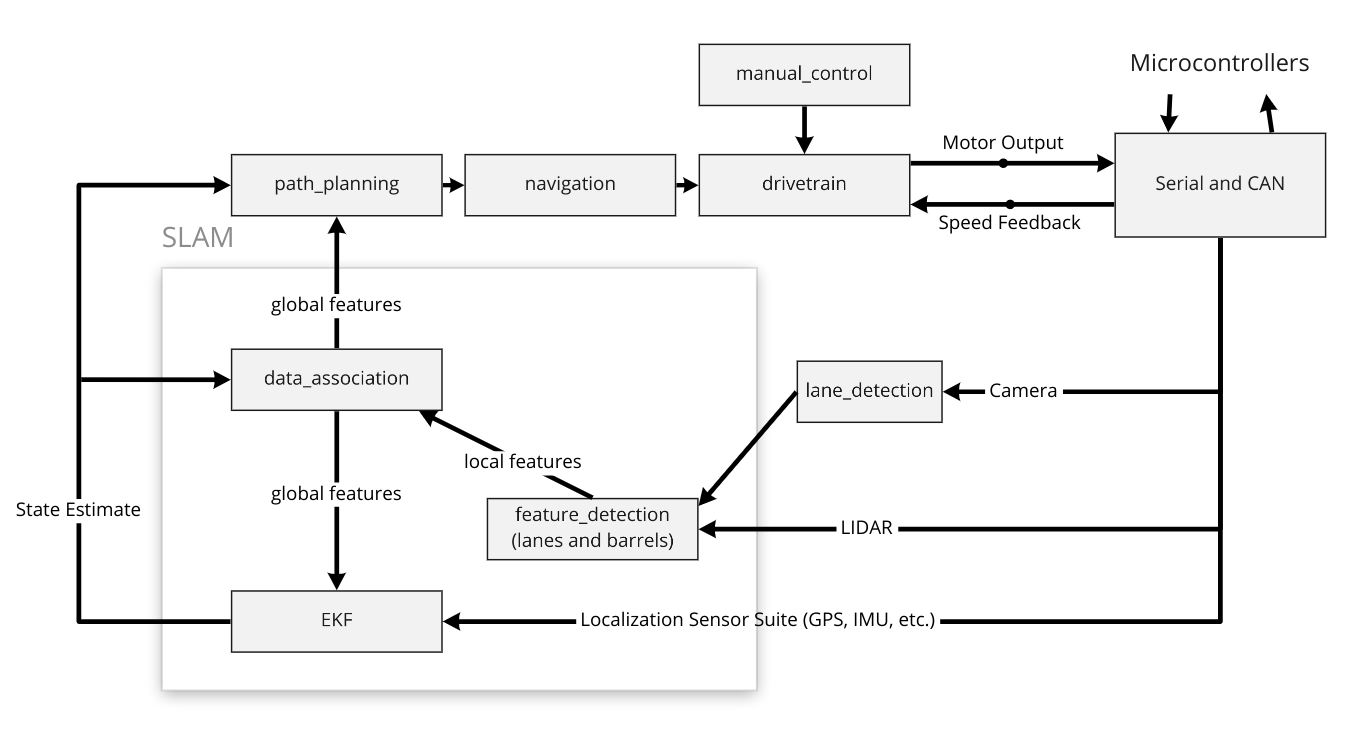
\includegraphics[width=0.9\textwidth]{images/software/software_block.png}
    \caption{Our software block diagram.}
    \label{fig:block:software}
\end{figure}

\subsection{Lane Detection}

To accomplish the difficult task of detecting the lanes, we experimented with two methods. The first method involved using standard computer vision techniques, and the second method was a convolutional neural network (CNN). Both ways perform the same overall function of taking an RGB image from the robot's Kinect camera and creating a black and white image with white identifying the lanes. 

Additionally, we perform a simple perspective correction to transform the image to a bird's eye view perspective. This allows us to directly use the image in the path planning step as described later.

\subsubsection{Computer Vision Techniques}

Our computer vision method used a variety of techniques chained together to produce our lane-segmented image. This consisted of applying thresholds to the HSV values to target pixels that match those of the lanes. This method was alright, but it was hard to find the balance between complexity in design and oversimplification of the results.

\subsubsection{Convolutional Neural Network}

Our second attempt used a convolutional neural network to detect lanes. The architecture we chose is a standard U-Net architecture which performs image segmentation well \cite{UNet}. We implemented the architecture in TensorFlow as it is easy to create models in and adjust to our needs quickly. We collected video of chalked grass using our robot's camera and then labeled the lane pixels in each image by hand to train the model. We then trained the model on these images, and we were able to produce the following results.

\begin{figure}[h]
    \centering
    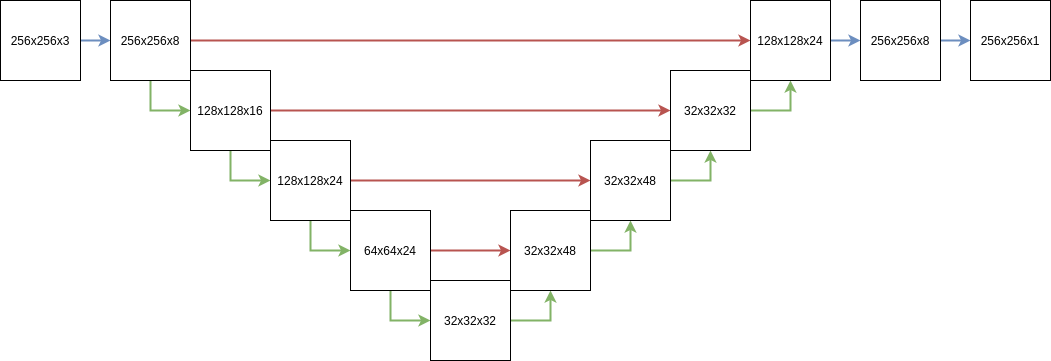
\includegraphics[width=0.7\textwidth]{images/software/unet.png}
    \caption{Our U-Net architecture which takes RGB images and outputs a black and white image of where the lanes are.}
\end{figure}

To ensure the CNN did not develop a simple thresholding algorithm, we took several different datasets in different weather conditions, with differently colored obstacles, and with people in the frame. The CNN succeeding with this amalgam of training data gives us high confidence that it will successfully identify all lanes and only lanes for most reasonable weather and brightness conditions.

\begin{figure}[H]
    \centering
    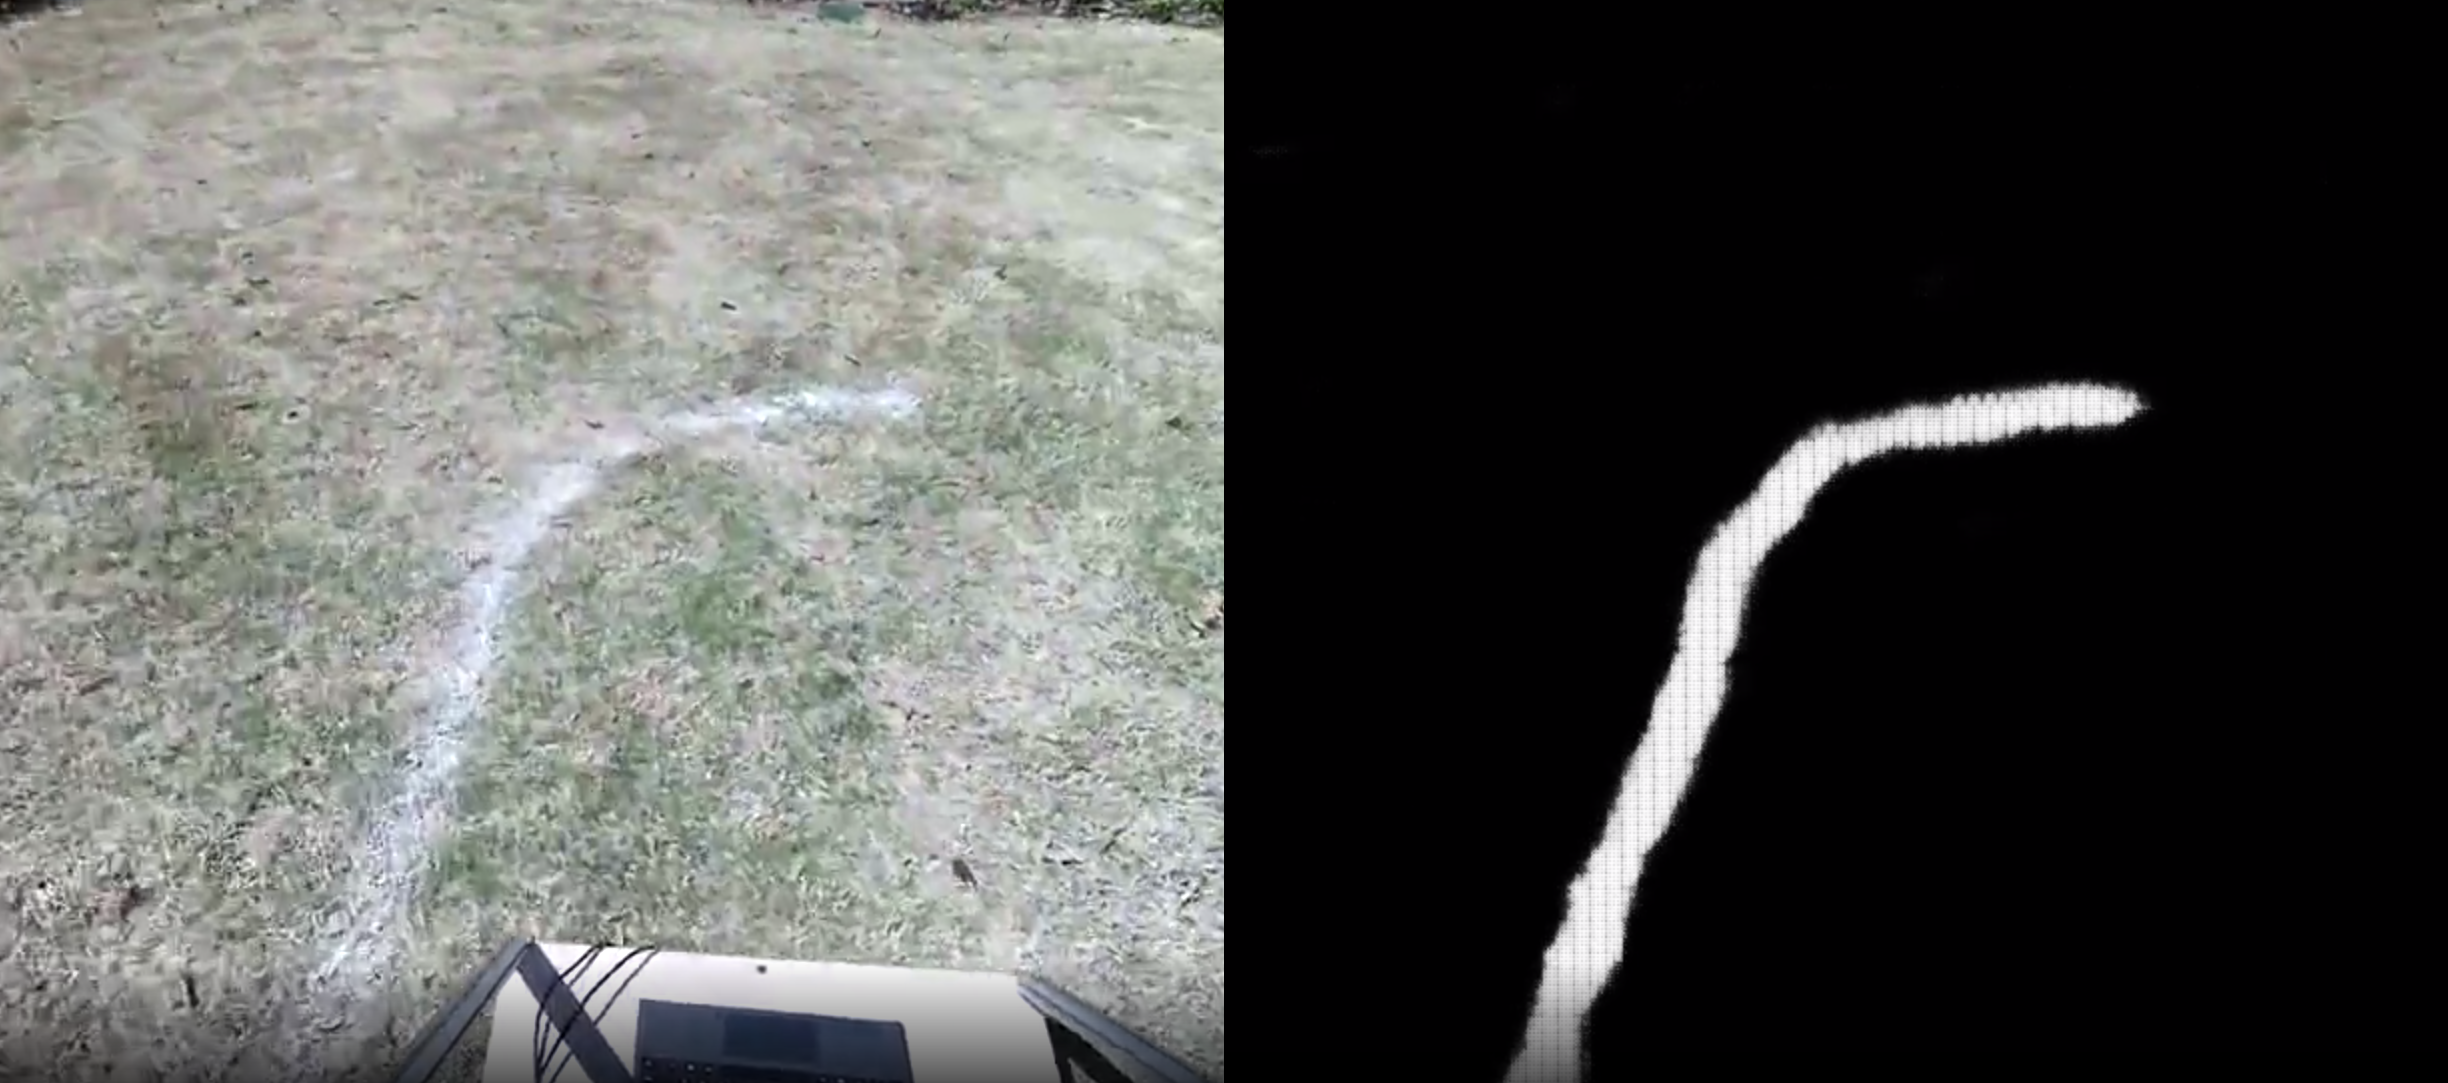
\includegraphics[width=0.5\textwidth]{images/software/unetexample.png}
    \caption{Cropped example showing the output of our U-Net on an image.}
\end{figure}

\subsection{Localization}

We use an Extended Kalman Filter (EKF) to track and update our \textit{state} estimation at every timestep. A Kalman Filter is a sensor fusion algorithm that performs a weighted average over time to balance measurements and predictions to track some state variables accurately. Our state, $\boldsymbol{X}$, consists of all variables we want to keep track of, plus all variables necessary to update the former. The state is a column vector,

\begin{equation}
    \boldsymbol{X} = \begin{pmatrix}
    x & \dot{x} & y & \dot{y} & \phi & \dot{\phi} & v_l & v_r
    \end{pmatrix} ^T
    \textrm{ ,}
    \label{eqn:kf:X}
\end{equation}
where $x$ and $y$ are the component positions in meters, $\dot{x}$ and $\dot{y}$ are the component velocities in meters per second, $\phi$ is the global heading (yaw) in degrees, $\dot{\phi}$ is the yaw rate, and $v_l$ and $v_r$ are the angular velocities of each wheel. 

To create and update this state, we receive input from several different sensors on our robot. We have available GPS, IMU, LiDAR, camera, and encoder data and choose only to use a subset of these. The reason is that for our use case, the EKF will only really come into play once we reach No Man's Land, so it isn't our highest priority. The measurement vector that we track each timestep is represented in Equation
(\ref{eqn:kf:Z}). It is possible to obtain and update our state with as little data as the wheel angular velocities and the yaw.

\begin{equation}
    \boldsymbol{Z} = \begin{pmatrix}
    v_l & v_r & \phi
    \end{pmatrix} ^T
    \label{eqn:kf:Z}
\end{equation}

We convert measurements to equivalent state values via Equation (\ref{eqn:kf:dynamics}). Note that we use a constant velocity model; this means the EKF assumes the velocity is constant, and any deviation from this is noise. The measurements will prod the correct evolution in these values, so this simplification works just fine.

\begin{equation}
    v = \frac{1}{2} \cdot \textrm{WHEEL\_RADIUS} \cdot (v_l + v_r)
    \label{eqn:kf:dynamics}
\end{equation}

\begin{equation*}
    \begin{cases}
    x = x + \dot{x} \Delta t\\
    \dot{x} = v \cos{\phi}\\
    y = y + \dot{y} \Delta t\\
    \dot{y} = v \sin{\phi}\\
    \phi = \phi - \dot{\phi} \Delta t\\
    \dot{\phi} = \frac{\textrm{WHEEL\_RADIUS}}{\textrm{WHEELBASE\_LEN}} \cdot (v_l - v_r)\\
    v_l = v_l\\
    v_r = v_r
    \end{cases}
\end{equation*}

The true benefit of the EKF comes when we dynamically increase the size of the state during landmark detection (from the LiDAR data). We add the $x$ and $y$ coordinates of the center of each landmark to the state and track this throughout the rest of the EKF runs. When we identify an obstacle, we can either add new values to the state or update existing values if we determine this landmark has been seen before. Landmarks, in this case, are primarily the traffic barrels that clutter the course and No Man's Land. 

When a new obstacle is added, we can assume it has no covariance with any other variables already in the state. This makes dynamicism very simple, as our Jacobian matrix will look the same, plus two additional rows and columns; all new entries other than the 2x2 in the lower right corner will be zero, and all existing entries are unaffected. 

The Jacobian is used when updating the state at each timestep and calculating the \textit{Innovation}, the difference between our predicted state and the new measurements. We create the initial Jacobian for our state using the Python package SymPy that is very good at symbolic calculations. We can make some assumptions about the covariance of each $i$th landmark's $x_i$ and $y_i$ positions, informed by our values for the robot's $x$ and $y$ in our original state. This is very helpful for computation time because we can manually create a new Jacobian when necessary rather than recreating it from scratch using SymPy and converting the symbolic representation to equations in our C++ node.

\subsection{Path Planning and Navigation}

Our goal is to navigate the course by sending control signals determined by the data from our sensors. Because it is our first year at this competition and we have much to learn, we decided to focus on building a robust and straightforward path planning and navigation system rather than using more complex algorithms. We hope to enhance this portion of our software design significantly in future years.

\subsubsection{Path Planning}

Our robot begins its decision-making process by taking in all the filtered sensor data. We take the laserscan data from the LiDAR and the detected lanes from our CNN, and combine them into a 2D occupancy grid detailing where the robot should not move. We then further transform this grid by marking each cell within a specified distance of an obstacle as occupied. This gives us a configuration space grid that lets us treat our robot as a single point to use standard path planning algorithms on this map without worrying about our robot getting too close to an obstacle. Finally, we run D* Lite on the final grid to give us a path from where the robot currently is to an ``ideal'' position \cite{DStar}. The ideal location is chosen by spotting a specified distance forward that is not inside an occupied grid space. As a result, our robot can only progress through the course and does not retain a memory of the overall course or where it has been, another feature we plan on improving significantly next year.

As a simplification to the EKF, we reset its state every time a new path is being planned, so that all positions and landmarks are tracked only for these small subpaths. This increases the accuracy at the cost of relying a bit more on the reactive behavior of the robot.

\subsubsection{Navigation}

Now that we have the path to follow, we have to create instructions for the robot to follow. To solve this, we used a simple path tracking algorithm called Pure Pursuit \cite{Pure Pursuit}. The algorithm takes the current position of the robot and the path we wish to pursue as an ordered list of points. The result is a heading that the robot should target that aims at a point on the path some short distance away from the robot. Using that heading, we can then generate motor instructions for our robot to turn the robot to face the heading. The robot always attempts to move forward but will reduce forward velocity while rotating to fit the heading.
